\section{Analysis of the sine modeling  method}
The analysis of the sinus method consists of multiple parts: First the error threshold was computed, which will be used to determine the first absorption dip from each of the change of channels per change of frequency measurements.
Second, the change of channels per change of frequency was computed. 
Third, the actual resonance frequency for each measurement was computed with the relation of the second step of this part of the analysis.
Fourth, the combination of the measured magnetic fields and computed frequencies was used to compute the magnetic momentum of the proton in $^{19}$F and the gyromagnetic ratio of the proton in glycol and hydrogen.
\subsection{Error thresholds}
%  Although two different pure background measurements were recorded, they ended up replaced by the noise recorded during the measurements for the change of channel per change of frequency.
For the error thresholds, one has to take a closer look at the recorded data. The .csv files obtained during the experiment contain the maxima and minima of the curves seen on the oscilloscope. To get a limit which is useful to discriminate the data multiple preparatory steps were necessary: First the absolute values of the differences from two neighbouring background data points were computed and projected to the y axis. A Gaussian curve was fitted to this projection. The maximum of the fitted curve, subtracted from to the mean of the background data used for the projection was the lower error threshold.\par 
In comparison to the out sample or in sample of frequency background, the background during the actual measurement is the most representative, because it was obtained during the exact same conditions as the signal data.
After taking an initial look at the measurements used for the frequency difference per channel difference (as seen in fig. \ref{all_dx}), it was decided that a sufficient amount of background data points can be obtained from these measurements. 
\begin{figure}[h]
	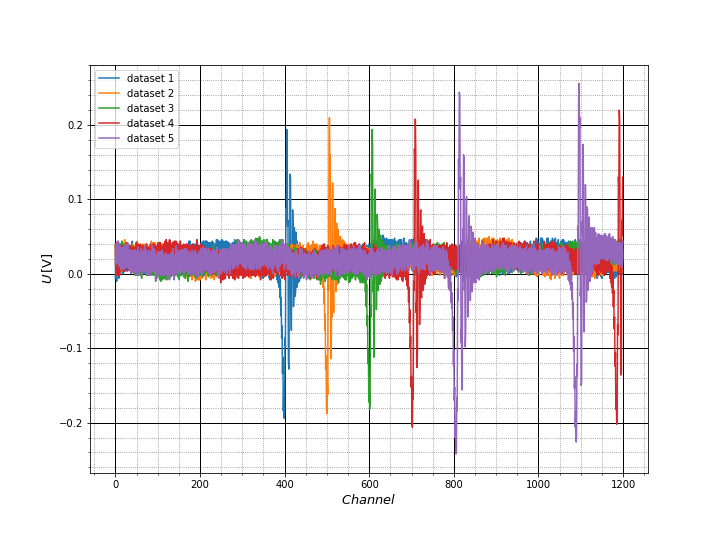
\includegraphics[scale=0.5]{Bild/all_dx.png}
	\centering
	\caption[Plot of all data used for the discriminator determination]{Plot of the measured voltage against the channel of the data points from all five measurements used for the difference in frequency per difference in channel.}
	\label{all_dx}
\end{figure}

After examining the first absorption peak of the first dataset, the parameter to coarsely seperate the background from the absorbtion signals was determined to be $-0.03\,$V. Both can be seen in fig. \ref{absorbtionpeak}. All values up to the tenth value underneath this threshold are considered as background signal.\par
\begin{figure}[h]
	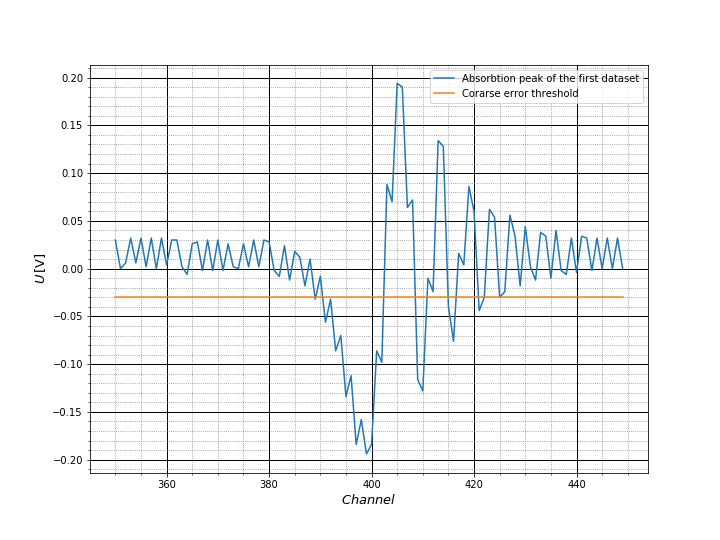
\includegraphics[scale=0.5]{Bild/peak_first_single.png}
	\centering
	\caption[Plot of an absorption peak]{Plot of the measured voltage against the channel of the absorption peak of the first measurement taken for the frequency change channel change ration measurement series. Also seen is the coarse error threshold of $-0.03\,$V.}
	\label{absorbtionpeak}
\end{figure}

All of these values can be seen in fig. \ref{all_err}. Now, the absolute difference between two neighbouring points was computed, which can be seen in fig. \ref{err_abs}. It is clearly visible, that all the data points in fig. \ref{all_err} and absolute differences in fig. \ref{err_abs} come in discrete levels. The reason behind this is the limited resolution of the analogue digital converter in the oscilloscope, which represents the values as binary numbers of a certain length, allowing only discrete voltage levels to be displayed. \par
These discrete levels result in zeros in the projection of the values to the y axis, which were not included in the fit of the Gaussian curve. 
The variance of the fitted Gaussian curve then was subtracted from the mean value of the background data, resulting in the lower error threshold.

\subsection{Computation of the relationship between a change in channels and a change in frequency}
For the coherence between the channels and the frequency, the absorption peaks of the five measurements were fitted to Gaussian curves. For this, the data below the error threshold of the first dip was used, ignoring the others as results of relaxation effects. After this, the first dip was chosen as the reference to compute the absolute difference between this one and all the other ones. 
The resulting linear relationship between the change in channels for the change of frequency can be seen in figure \ref{dx/df}.

\subsection{Computation of the resonance frequencies}
With the computed error threshold and channel frequency relationship, the resonance frequencies of the different samples can be computed.
For this, the nullstellen of the magnetic field modifying sine wave were computed, utilizing a sine fit with \verb|curve_fit|. Next, the resonance signal next to the nullstellen was analysed for the absorption maxima. Utilizing the error threshold, all values above were considered background. From the data points left the first dip was recorded to be analysed. Caused by the low sample number in the files, the original plan of fitting a Gaussian curve to each dip was not feasible. As a substitute, the minimum of each dip was chosen to be the recorded channel with the width of the entire dip as the error. This can be seen in figure \ref{dip_points}
Now, the distance between the dip and the closest nullstelle of the sine was computed for all dip-nullstellen pairs in the measurement and the mean of all distances was computed. This mean is the correction  for the frequency at which the measurement was recorded. Utilizing the frequency channel relationship, the true resonance frequency of each measurement could be computed as the sum of the recorded frequency and the correction.


\subsection{Computation of the nuclear magnetic momentum of $^9$F}
Using the corrected resonance frequencies and measured magnetic fields, the gyromagnetic ratio and nuclear magnetic momentum of $^9$F were computed. Due to time dependent changes of the magnetic field, the error of the measured magnetic field was set to $\Delta B = 1\,\text{mT}$. The resonance frequency has been corrected using the above steps. Utilizing the formular \ref{important_formular}, formulars \ref{formel_gamma} and \ref{formular_mu} could be deduced. $\hbar$ does not have an error, for it is a fundamental constant \cite{hbar}.
\begin{equation}
	\label{formel_gamma}
	\gamma = 2 \pi \frac{\nu_{res}}{B};\qquad \Delta\gamma = \gamma \sqrt{\left(\frac{\delta\nu_{res}}{\nu_{res}}\right)^2 + \left(\frac{\Delta B}{B}\right)^2}
\end{equation}
\begin{equation}
\label{formular_mu}
	\mu_K = \gamma\hbar\m_I = \frac{\gamma\hbar}{2}, \qquad \Delta \mu_K = \mu_K \left(\frac{\Delta \gamma}{\gamma}\right)
\end{equation}
\begin{table}[h]
	\caption{Calculated results of $^9$F}
	\label{teflon}
	\begin{tabular}{lllll}
		\toprule
		{} & Corrected resonance frequencies & Measured magnetic fields &           $\gamma$ &                $\mu_K$ \\
		\midrule
		0 &                  19.096+/-0.006 &              461.0+/-1.0 &  0.2603+/-0.0006 &  (1.3724+/-0.0030)e-35 \\
		1 &                  19.496+/-0.005 &              503.0+/-1.0 &  0.2435+/-0.0005 &  (1.2841+/-0.0026)e-35 \\
		2 &                  18.524+/-0.006 &              474.0+/-1.0 &  0.2456+/-0.0005 &  (1.2948+/-0.0028)e-35 \\
		3 &                  17.999+/-0.006 &              436.0+/-1.0 &  0.2594+/-0.0006 &  (1.3677+/-0.0032)e-35 \\
		4 &                  17.548+/-0.006 &              447.0+/-1.0 &  0.2467+/-0.0006 &  (1.3006+/-0.0029)e-35 \\
		5 &                  18.022+/-0.006 &              466.0+/-1.0 &  0.2430+/-0.0005 &  (1.2813+/-0.0028)e-35 \\
		\bottomrule
	\end{tabular}

\end{table}
\subsection{Computation of the gyromagnetic ratio of the proton}

Analogue to the previous calculation, the gyromagnetic ratio of the proton in glycol and hydrogen was computed with formular \ref{formel_gamma}. The results are seen in table \ref{glycol} for the glycol sample and table \ref{hydrogen} for hydrogen. 
\begin{table}[h]
	\caption{Calculated results of Glycol}
	\label{glycol}
	\begin{tabular}{llll}
		\toprule
		{} & Corrected resonance frequencies [Mhz] & Measured magnetic fields [mT] &               \$\textbackslash gamma\$ \\
		\midrule
		0 &                        18.577+/-0.006 &                           395 &  (2.9550+/-0.0009)e+08 \\
		1 &                        18.079+/-0.007 &                           383 &  (2.9660+/-0.0012)e+08 \\
		2 &                        17.520+/-0.006 &                           371 &  (2.9671+/-0.0009)e+08 \\
		3 &                        19.039+/-0.006 &                           405 &  (2.9537+/-0.0009)e+08 \\
		4 &                        19.492+/-0.006 &                           414 &  (2.9582+/-0.0008)e+08 \\
		\bottomrule
	\end{tabular}
\end{table}

\begin{table}
	\caption{Calculated results of hydrogen}
	\label{hydrogen}
	\begin{tabular}{llll}
		\toprule
		{} & Corrected resonance frequencies [Mhz] & Measured magnetic fields [mT] &               \$\textbackslash gamma\$ \\
		\midrule
		0 &                        19.560+/-0.006 &                           414 &  (2.9686+/-0.0008)e+08 \\
		1 &                        19.678+/-0.005 &                           418 &  (2.9579+/-0.0008)e+08 \\
		2 &                        19.002+/-0.006 &                           404 &  (2.9552+/-0.0009)e+08 \\
		3 &                        18.151+/-0.006 &                           380 &  (3.0012+/-0.0009)e+08 \\
		4 &                        17.519+/-0.006 &                           371 &  (2.9670+/-0.0010)e+08 \\
		5 &                        18.649+/-0.006 &                           397 &  (2.9515+/-0.0009)e+08 \\
		\bottomrule
	\end{tabular}
\end{table}